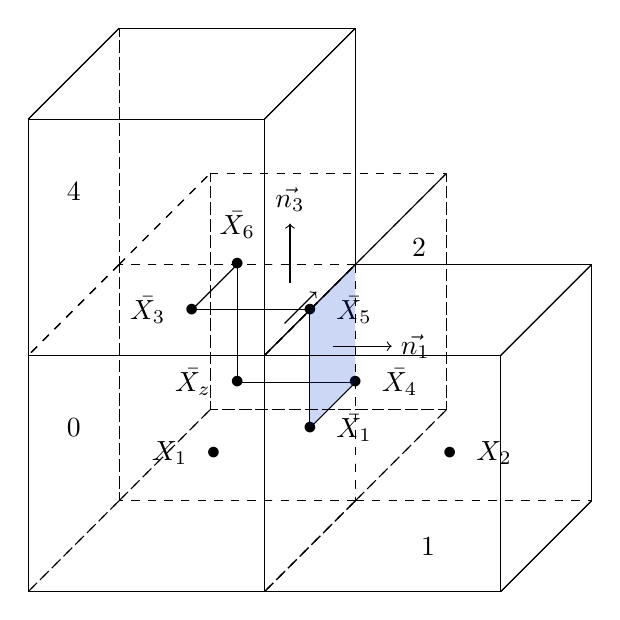
\begin{tikzpicture}[scale = 3, cm={1,0,-1,-1, (0,0)},y=-3.85mm, z = -1cm]

\node at (-1,-0.5,0.5) {$4$};
\node at (0,0.7,-0.2)  {$2$};
\node at (-1,-0.5,-0.5){$0$};
\node at (0.5,-0.5,-1) {$1$};
\node[label=left:$X_1$] at (-0.6,0,-0.8) {$\bullet$};
\node[label=right:$X_2$] at (0.4,0,-0.8)  {$\bullet$};
\node[label=left:$\bar{X_3}$] at (-0.5,-0.5,0)  {$\bullet$};
\node[label=above:$\bar{X_6}$] at (-0.5,0,0)  {$\bullet$};
\node[label=right:$\bar{X_5}$] at (0,-0.5,0)  {$\bullet$};
\node[label=left:$\bar{X_z}$] at (-0.5,0,-0.5)  {$\bullet$};
\node[label=right:$\bar{X_1}$] at (0,-0.5,-0.5)  {$\bullet$};
\node[label=right:$\bar{X_4}$] at (0,0,-0.5)  {$\bullet$};

%Area

\draw[] (-0.5,0,0)    -- (-0.5,-0.5,0);
\draw[] (-0.5,-0.5,0) -- (0,-0.5,0);
\draw[] (0,-0.5,0)    -- (0,-0.5,-0.5);
\draw[] (0,-0.5,-0.5) -- (0,0,-0.5);
\draw[] (0,0,-0.5)    -- (-0.5,0,-0.5);
\draw[] (-0.5,0,-0.5) -- (-0.5,0,0);

\definecolor{lila}{rgb}{0,0.2,0.8}
\begin{scope}
  \clip[postaction={fill=lila,fill opacity=0.2}](0,0,0) -- (0,-0.5,0) -- (0,-0.5,-0.5) -- (0,0,-0.5) -- (0,0,0);
\end{scope}

%Arrows
\draw[->] (-0.2,-0.2,0) -- (-0.2,-0.2,0.25);
\node at  (-0.2,-0.2,0.35) {$\vec{n_3}$};
\draw [->](0,-0.25,-0.25) -- (0.25,-0.25,-0.25);
\node at  (0.35,-0.25,-0.25) {$\vec{n_1}$};
\draw [->](-0.3,0,-0.25) -- (-0.3,0.35,-0.25);

%Cube Left Front Upper

%X-Y rectangle Z = 1
\draw[] (-1,-1,1) -- (0,-1,1);
\draw[] (0,-1,1)  -- (0,0,1);
\draw[] (0,0,1)   -- (-1,0,1);
\draw[] (-1,0,1)  -- (-1,-1,1);

%X-Z rectangle Y = -1
\draw[] (-1,-1,1) -- (-1,-1,0);
\draw[] (-1,-1,0) -- (0,-1,0);
\draw[] (0,-1,0)  -- (0,-1,1);
\draw[] (0,-1,1)  -- (-1,-1,1);

%Z-Y rectangle X = 0
\draw[] (0,-1,1) -- (0,-1,0);
\draw[] (0,-1,0) -- (0,0,0);
\draw[] (0,0,0)  -- (0,0,1);
\draw[]  (0,0,1) -- (0,-1,1);

%X-Y rectangle Z = 0
\draw[] (-1,-1,0) -- (0,-1,0);
\draw[dashed] (0,-1,0) -- (0,0,0);
\draw[dashed] (0,0,0)  -- (-1,0,0);
\draw[dashed] (-1,0,0) -- (-1,-1,0);

%Y-Z rectangle X = -1
\draw[] (-1,-1,0) -- (-1,-1,1);
\draw[] (-1,-1,1) -- (-1,0,1);
\draw[dashed] (-1,0,1) -- (-1,0,0);
\draw[dashed] (-1,0,0) -- (-1,-1,0);

%X-Z rectangle Y = 0
\draw[dashed] (0,0,0)  -- (-1,0,0);
\draw[dashed] (-1,0,0) -- (-1,0,1);
\draw[dashed] (0,0,0)  -- (0,0,1);
\draw[]       (0,0,1)  -- (-1,0,1);

%Cube Left Front Lower

%X-Y rectangle Z = -1
\draw[] (-1,-1,-1) -- (0,-1,-1);
\draw[dashed] (0,-1,-1)  -- (0,0,-1);
\draw[dashed] (0,0,-1)   -- (-1,0,-1);
\draw[dashed] (-1,0,-1)  -- (-1,-1,-1);

%X-Z rectangle Y = -1
\draw[] (-1,-1,-1) -- (-1,-1,0);
\draw[] (-1,-1,0) -- (0,-1,0);
\draw[] (0,-1,0)  -- (0,-1,-1);
\draw[] (0,-1,-1)  -- (-1,-1,-1);

%Z-Y rectangle X = 0
\draw[] (0,-1,-1) -- (0,-1,0);
\draw[dashed] (0,-1,0) -- (0,0,0);
\draw[dashed] (0,0,0)  -- (0,0,-1);
\draw[dashed]  (0,0,-1) -- (0,-1,-1);

%X-Y rectangle Z = 0
\draw[] (-1,-1,0) -- (0,-1,0);
\draw[dashed] (0,-1,0) -- (0,0,0);
\draw[dashed] (0,0,0)  -- (-1,0,0);
\draw[dashed] (-1,0,0) -- (-1,-1,0);

%Y-Z rectangle X = -1
\draw[] (-1,-1,0) -- (-1,-1,-1);
\draw[dashed] (-1,-1,-1) -- (-1,0,-1);
\draw[dashed] (-1,0,-1) -- (-1,0,0);
\draw[dashed] (-1,0,0) -- (-1,-1,0);

%X-Z rectangle Y = 0
\draw[dashed] (0,0,0)  -- (-1,0,0);
\draw[dashed] (-1,0,0) -- (-1,0,-1);
\draw[dashed] (0,0,0)  -- (0,0,-1);
\draw[dashed]       (0,0,-1)  -- (-1,0,-1);

%Cube Right Front Lower

%X-Y rectangle Z = -1
\draw[] (1,-1,-1) -- (0,-1,-1);
\draw[dashed] (0,-1,-1)  -- (0,0,-1);
\draw[dashed] (0,0,-1)   -- (1,0,-1);
\draw[] (1,0,-1)  -- (1,-1,-1);

%rX-Z rectangle Y = -1
\draw[] (1,-1,-1) -- (1,-1,0);
\draw[] (1,-1,0) -- (0,-1,0);
\draw[] (0,-1,0)  -- (0,-1,-1);
\draw[] (0,-1,-1)  -- (1,-1,-1);

%Y-Z rectangle X = 0
\draw[] (0,-1,-1) -- (0,-1,0);
\draw[] (0,-1,0) -- (0,0,0);
\draw[dashed] (0,0,0)  -- (0,0,-1);
\draw[dashed]  (0,0,-1) -- (0,-1,-1);

%X-Y rectangle Z = 0
\draw[] (1,-1,0) -- (0,-1,0);
\draw[dashed] (0,-1,0) -- (0,0,0);
\draw[dashed] (0,0,0)  -- (1,0,0);
\draw[] (1,0,0) -- (1,-1,0);

%Y-Z rectangle X = 1
\draw[] (1,-1,0) -- (1,-1,-1);
\draw[] (1,-1,-1) -- (1,0,-1);
\draw[] (1,0,-1) -- (1,0,0);
\draw[] (1,0,0) -- (1,-1,0);

%X-Z rectangle Y = 0
\draw[] (0,0,0)  -- (1,0,0);
\draw[] (1,0,0) -- (1,0,-1);
\draw[dashed] (0,0,0)  -- (0,0,-1);
\draw[dashed] (0,0,-1)  -- (1,0,-1);

%Cube Left Back Lower

%X-Y rectangle Z = -1
\draw[dashed] (-1,1,-1) -- (0,1,-1);
\draw[dashed] (0,1,-1)  -- (0,0,-1);
\draw[dashed] (0,0,-1)   -- (-1,0,-1);
\draw[dashed] (-1,0,-1)  -- (-1,1,-1);

%X-Z rectangle Y = 1
\draw[dashed] (-1,1,-1) -- (-1,1,0);
\draw[dashed] (-1,1,0) -- (0,1,0);
\draw[dashed] (0,1,0)  -- (0,1,-1);
\draw[dashed] (0,1,-1)  -- (-1,1,-1);

%Y-Z rectangle X = 0
\draw[dashed] (0,1,-1) -- (0,1,0);
\draw[] (0,1,0) -- (0,0,0);
\draw[dashed] (0,0,0)  -- (0,0,-1);
\draw[dashed]  (0,0,-1) -- (0,1,-1);

%X-Y rectangle Z = 0
\draw[dashed] (-1,1,0) -- (0,1,0);
\draw[dashed] (0,1,0) -- (0,0,0);
\draw[dashed] (0,0,0)  -- (-1,0,0);
\draw[dashed] (-1,0,0) -- (-1,1,0);

%Y-Z rectangle X = -1
\draw[dashed] (-1,1,0) -- (-1,1,-1);
\draw[dashed] (-1,1,-1) -- (-1,0,-1);
\draw[dashed] (-1,0,-1) -- (-1,0,0);
\draw[dashed] (-1,0,0) -- (-1,1,0);

%X-Z rectangle Y = 0
\draw[dashed] (0,0,0)  -- (-1,0,0);
\draw[dashed] (-1,0,0) -- (-1,0,-1);
\draw[dashed] (0,0,0)  -- (0,0,-1);
\draw[dashed]       (0,0,-1)  -- (-1,0,-1);







\end{tikzpicture}